\documentclass[a4paper]{article}

\usepackage{cite}%多个文献引用
\usepackage{graphicx}
\usepackage{array}%调节表格行高
\usepackage{multirow,makecell}%多行表格
\usepackage{tabularx}%表格固定列宽
\usepackage{subfigure}
\usepackage{titlesec}%标题格式设置
\usepackage{amsmath}
\usepackage{amssymb}
\usepackage{tabularx}
\usepackage{makecell}
\usepackage{geometry}
\usepackage{float}
\usepackage{setspace}%行距包
\usepackage{siunitx}
\usepackage{mdwlist}
\usepackage{tabu}
\usepackage{enumerate}

\geometry{top=1.54cm,bottom=2.54cm,left=2.5cm,right=2.5cm}


\begin{document}
\begin{center}
\bf\Large
EE 105 Feedback Control Systems\par
Department of Electrical and Computer Engineering\par
Tufts University Fall 2018\par
Homework \#6\par   
\end{center}
\begin{table}[H]
\begin{center}
\begin{tabular*}{\textwidth}{@{\extracolsep{\fill}}lcr}
Name: {\it Shang Wang} &Student ID: {\it 1277417} &E-mail: {\it shang.wang@tufts.edu}\\
\hline
\end{tabular*}
\end{center}
\end{table}

\section{Problem 1}
\subsection{Part A} 
The transfer function is:
$$
G(s) = \frac{100}{(s+0.1)(s+1)}
$$
So the step response is:
\begin{figure}[H]
\centering
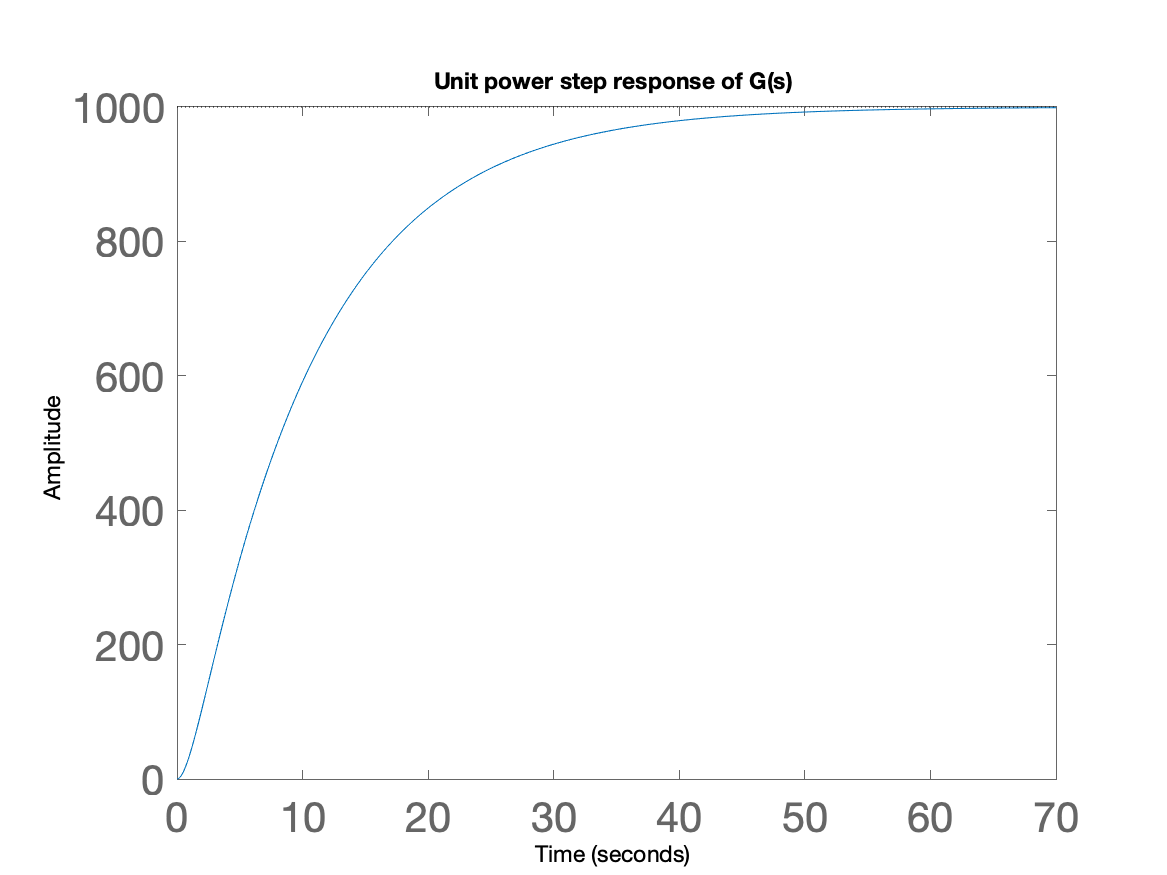
\includegraphics[width = 0.6\textwidth]{pic/t1.png}
\end{figure}

\subsection{Part B} 
Root locus of the system with proportional control only:
\begin{figure}[H]
\centering
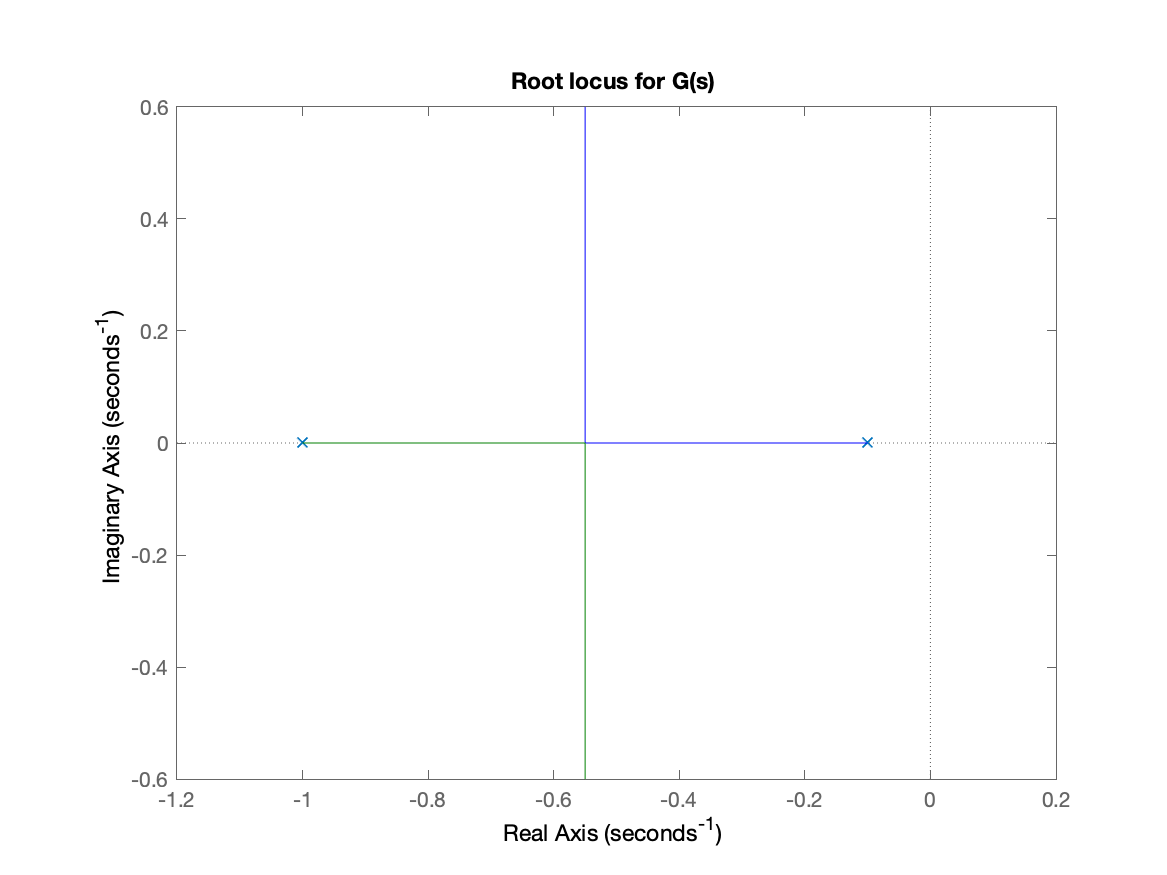
\includegraphics[width = 0.6\textwidth]{pic/t2.png}
\end{figure}

\subsection{Part C} 
Adjust the gain to high enough to meet the rise time specification ($t_r < 1 s$):
$$
K = 0.2
$$
The transfer function is:
$$
P(s)  =\frac{100KG(s)}{1+100KG(s)} = \frac{K'G(s)}{1+K'G(s)}
$$
The step response is:
\begin{figure}[H]
\centering
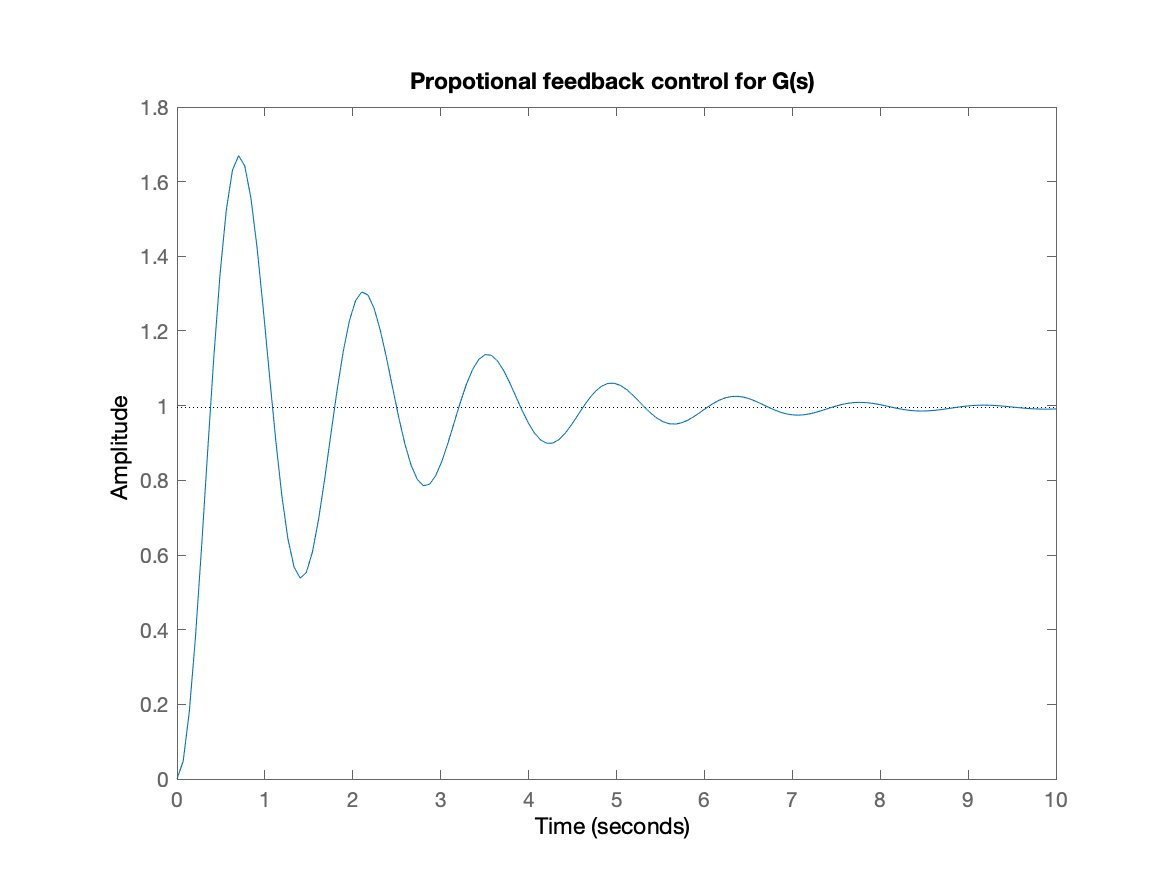
\includegraphics[width = 0.6\textwidth]{pic/t3.png}
\end{figure}

\subsection{Part D} 
If required a system with none steady error to a step, we need to design the lag compansator with zero pole to make a open loop transfer function a type one transfer function. Since we always have no idea about the complete dynamics of such a thermadynamic system, we can not accurately cancel a poles by applying some lead or lag controller. Thus our open loop transfer function $H(s) = D(s)G(s)$ will become:
$$
H(s) = K'\frac{1}{(s+1)(s+0.1)}\cdot\frac{s+2}{s+13}\cdot\frac{s+0.04}{s}
$$
The root locus of $H(s)$ is(where $K' = 30$):
\begin{figure}[H]
\centering
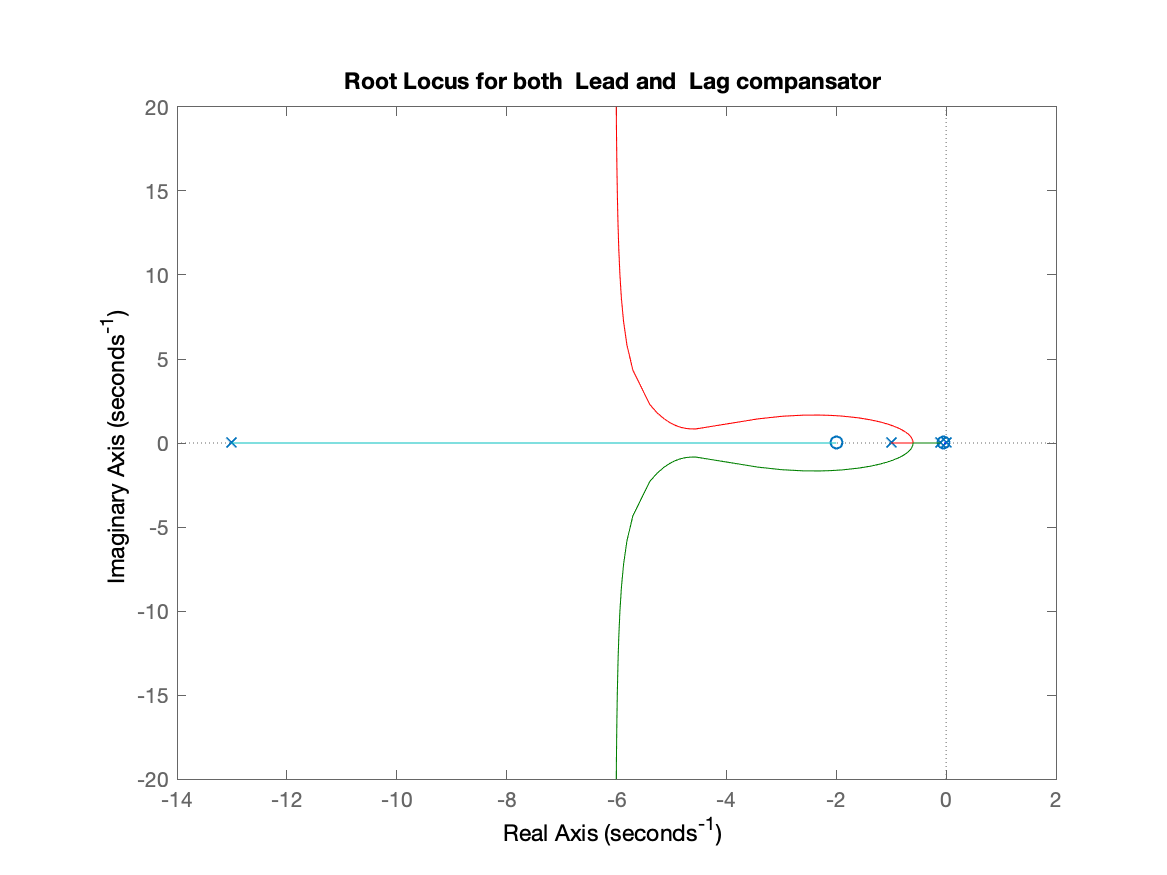
\includegraphics[width = 0.6\textwidth]{pic/t4.png}
\end{figure}
Response to a step:
\begin{figure}[H]
\centering
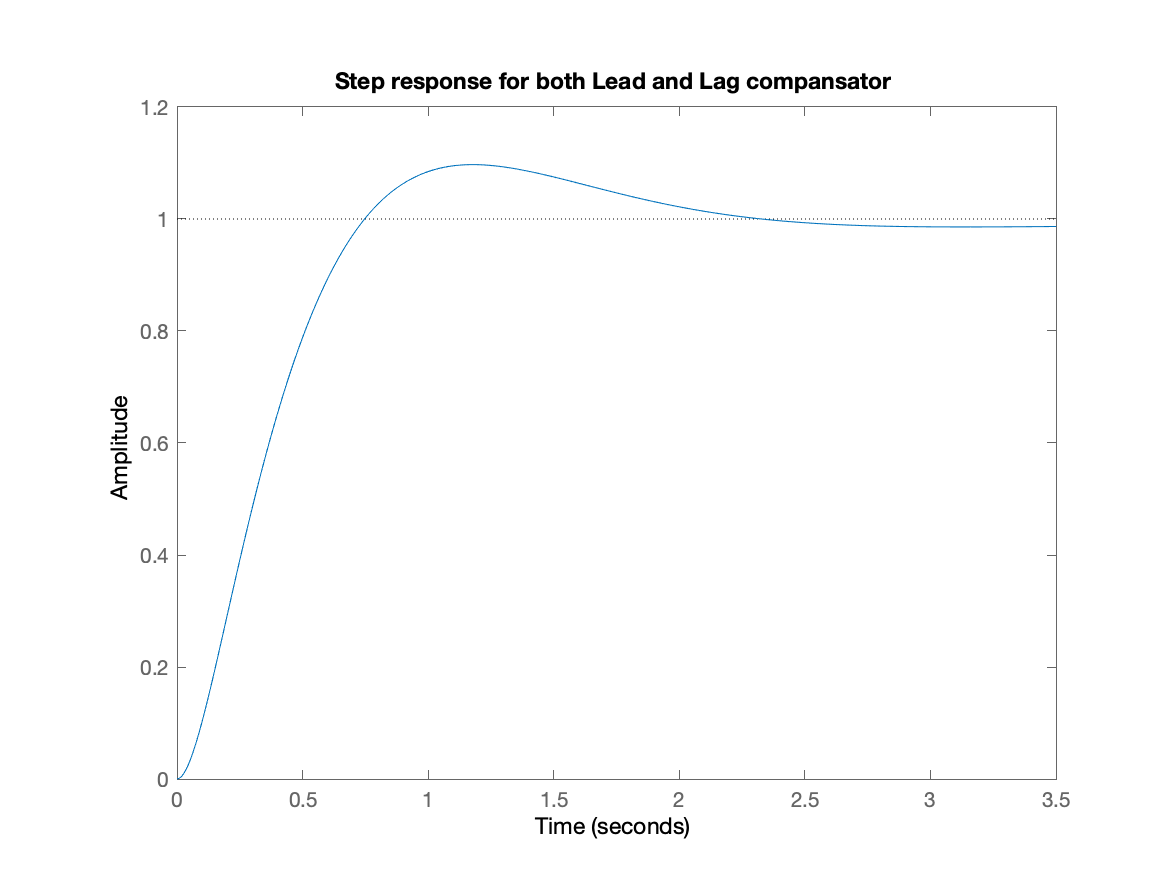
\includegraphics[width = 0.6\textwidth]{pic/t5.png}
\end{figure}

\subsection{Part E} 
While applying a lag compensator $D_{lag} = (s+0.04)/s$, which will add a really slow decay term in the transfer function of time domain. That's where the small tail come from.  

\begin{figure}[H]
\centering
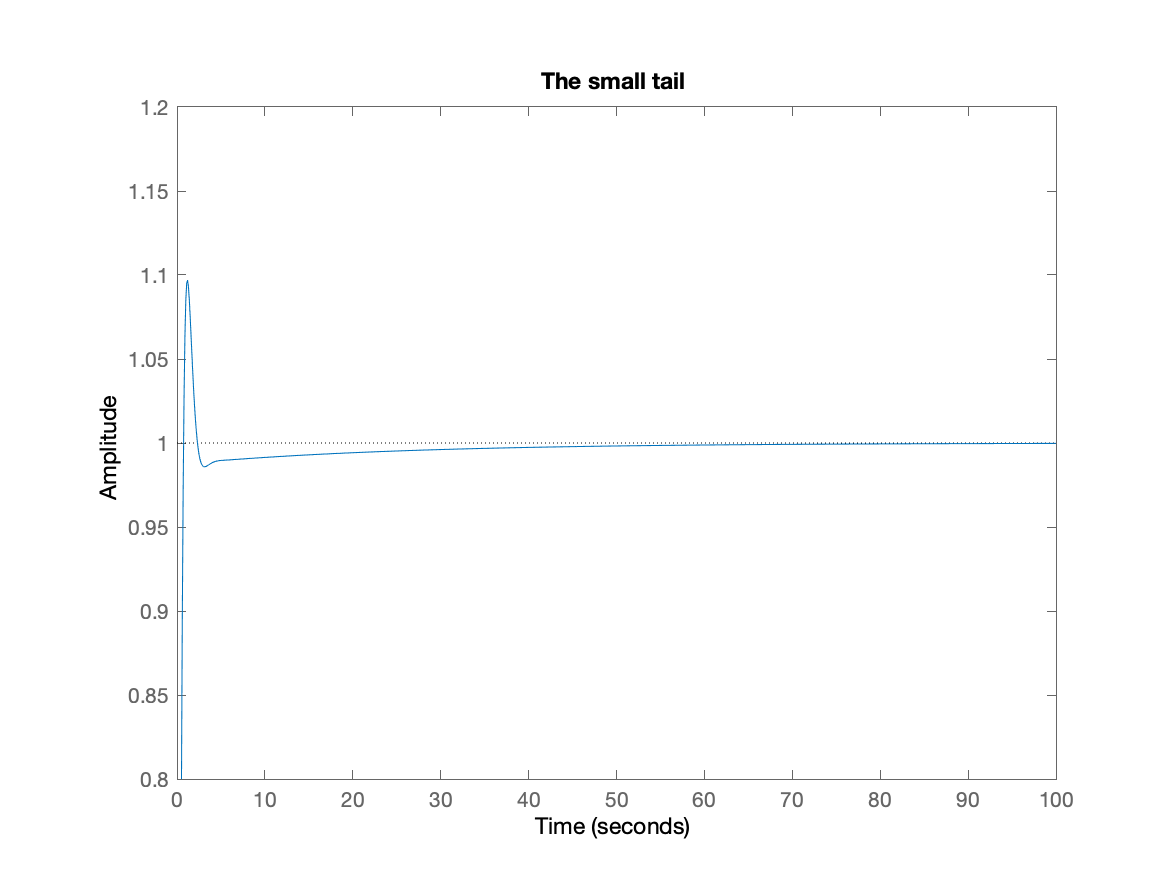
\includegraphics[width = 0.6\textwidth]{pic/t6.png}
\end{figure}


% \begin{figure}[H]
% \centering
% 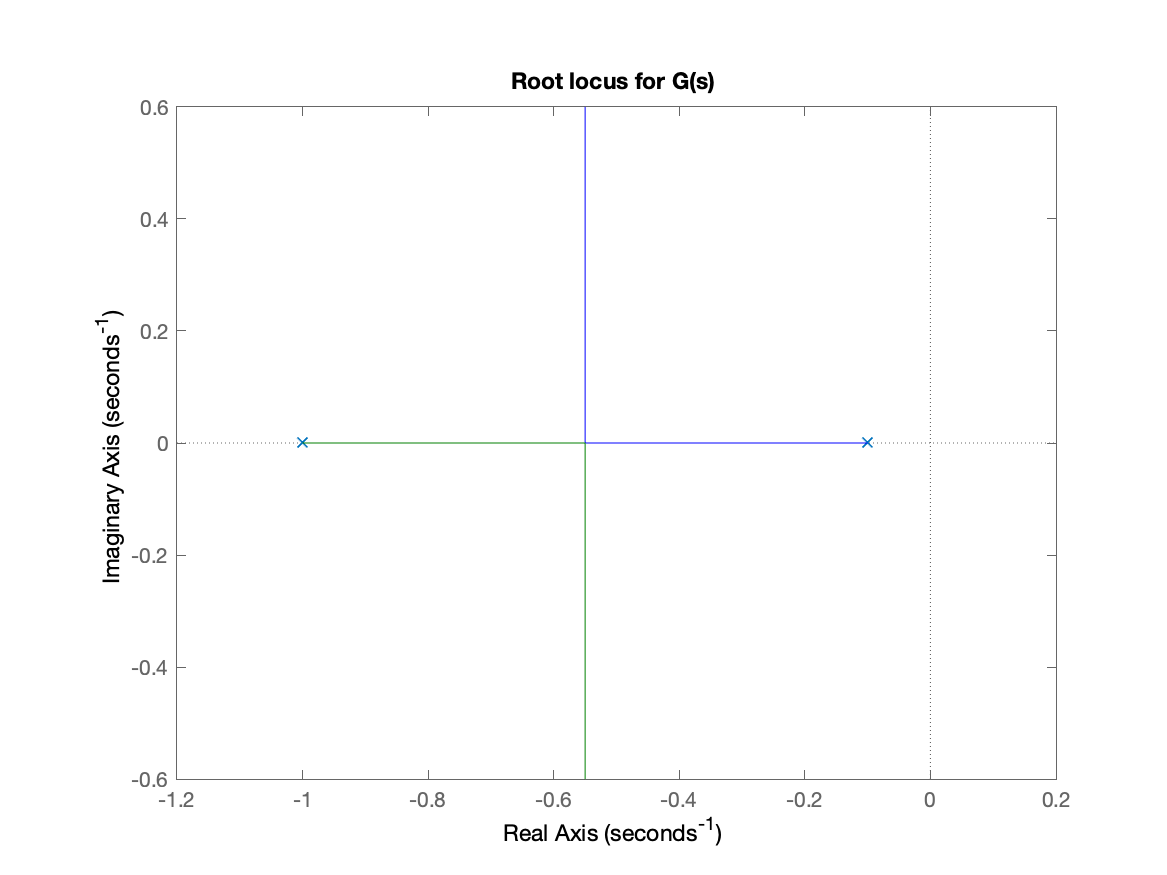
\includegraphics[width = 0.6\textwidth]{pic/t2.png}
% \end{figure}



\end{document}